%-----------------------------------------------------------------------------%
\chapter{\babDua}
%-----------------------------------------------------------------------------%
Pada bab ini menjelaskan tentang tinjauan pustaka yang digunakan sebagai landasan penelitian.
Penjelasan tersebut antara lain mengenai \f{user experience}, \f{e-government},
\f{usability}, \f{usability testing}, \f{prototyping} serta \f{website} Direktorat Jenderal Pajak Indonesia dan India.
%-----------------------------------------------------------------------------%

\section{\f{Human Computer Interaction}}
\f{Human Computer Interaction} (HCI) adalah bidang dalam ilmu komputer yang mempelajari bagian desain sistem yang berinteraksi langsung dengan pengguna. Ilmu ini berkembang dari kebutuhan dalam pemahaman terkait kemudahan dan kenyamanan menggunakan suatu produk perangkat lunak oleh pengguna. HCI sendiri dibagi kedalam 2 aspek, yaitu \f{functionality} dan \f{usability} \citep{}. 
%-----------------------------------------------------------------------------%
\subsection{\f{User Experience}}
\f{User experienc} atau disingkat UX merupakan salah satu aspek penting dalam mengembangkan suatu produk. Ilmu terkait UX sendiri sudah berkembang dari pertengahan tahun 1990-an. Interaksi antara pengguna dengan produk merupakan salah satu cakupan dari aspek UX. Definisi \f{User Experience} menurut ISO 9241-210 adalah persfektif seseorang terhadap penggunaan dari suatu produk, sistem atau layanan \citet{}. Sedangkan menurut \citet{} User Experience adalah kepuasan secara menyeluruh seorang pengguna dari hasil interaksi dengan sebuah produk atau alat digital. \citet{} menyebutkan bahwa \f{user experience} adalah pengalaman yang diciptakan oleh produk kepada pengguna yang menggunakannya di dunia nyata.
Terdapat beberapa definisi mengenai \f{User Experience}, namun semua rujukan tersebut menuju sebuah tujuan yaitu pengalaman pengguna terhadap penggunaan suatu produk, dengan artian produk apapun tanpa terkecuali sistem aplikasi baik berbentuk \f{website} ataupun \f{desktop}.
\newline\\
\citet{} menjelaskan dalam bukunya yang berjudul "" bahwa UX terbagi menjadi 7 aspek. Ketujuh aspek tersebut adalah sebagai berikut.
\begin{enumerate}
	\item \f{Useful}, yaitu bermanfaat bagi pengguna.
	\item \f{Usable}, yaitu dapat dengan mudah digunakan pengguna.
	\item \f{Desireable}, yaitu memiliki elemen desain yang membangkitkan emosi dan apresiasi pengguna.
	\item \f{Findable}, yaitu kemudahan dalam pencarian konten aplikasi.
	\item \f{Accessible}, yaitu konten aplikasi dapat dengan mudah diakses pengguna. 
	\item \f{Credible}, yaitu konten aplikasi harus terpercaya.
	\item \f{Valuable}, yatu memiliki nilai yang memenuhi dan meningkatkan kepuasan pengguna.
\end{enumerate}
%-----------------------------------------------------------------------------%
\subsection{\f{Usability}}
\f{Usability} adalah kualitas yang menjadi penilaian bagaimana suatu tampilan antarmuka sistem dapat dengan mudah digunakan. Usability merupakan salah satu faktor penting dalam kesuksesan sitem komputer atau layanan berbasis komputer. Menurut citet{} \f{usability} menekankan kemudahan sistem untuk digunakan sesuai dengan tujuan sistem tersebut. Seperti membuat penambahan halaman pada dokumen, pengguna harus mengetaui dengan jelas apa yang perlu dilakukan serta melakukan aksi yang tidak banyak untuk mencapainya.
Banyak sekali definisi terkait dengan usability ini, namun bisa diketahui bahwa usability berkaitan erat dengan produk atau sistem dan peforma pengguna yang meliputi efektivitas, efisiensi, kemudahan dalam penggunaan serta pengalaman pengguna terkait produk atau sistem tersebut.
\newline\\
\citet{} mengemukakan bahwa terdapat 5 komponen utama terkait usability yang mudah digunakan pengguna atau disebut juga sebagai kategori user friendly. Berikut penjabaran terkait 5 komponen utama usability, yaitu:
\begin{enumerate}
	\item \f{Learnability}\\
	\f{Learnability} menjelaskan seberapa mudah aplikasi untuk dipelajari, dimengerti dan dipahami oleh pengguna ketika menggunakan produk pertama kali.
	\item \f{Efficiency}\\
	\f{Efficiency} merupakan komponen yang berkaitan dengan efisiensi menu-menu pada produk aplikasi sehingga pengguna dapat menggunakan produk secara cepat dan mudah.
	\item \f{Memorability}\\
	\f{Memorability} menjelaskan mengenai kemudahan pengguna untuk mengingat fungsi-fungsi yang terdapat pada produk aplikasi. Komponen \f{memorability} menjelaskan bahwa jika pengguna tidak menggunakan produk aplikasi dalam beberapa waktu maka ketika pengguna menggunakan produk aplikasi dapat dengan mudah menggunakannya tanpa mempelajari kembali produk aplikasi tersebut.
	\item \f{Error}\\
	\f{Error} merupakan kesalahan atau error yang dilakukan oleh pengguna ketika menggunakan produk sehingga pengguna dapat memperbaiki kesalahannya.
	\item \f{Satisfaction}\\
	\f{Satisfaction} merupakan tingkat kepuasan pengguna terhadap tampilan antarmuka dari produk aplikasi.
\end{enumerate}
Selain komponen yang dikemukakan \citeauthor{} diatas, terdapat juga pendapat lainnya mengenai komponen \f{usability}, seperti \citet{} yang mengemukakan terdapat 4 komponen dalam \f{usability} antara lain learnability, throughout, flexibility dan attitude. Sedangkan \citet{} mengemukakan bahwa usability memiliki fokus terhadap 3 komponen, yaitu easy to learn, easy to use dan kepuasan pengguna terhadap penggunaan sistem.
%-----------------------------------------------------------------------------%
\subsection{\f{Nielsen's Usability Heuristics}}
\citet{} mengemukakan 10 prinsip terkait desain interaksi. Kesepuluh prinsip tersebut merupakan usability "heuristic" karena berbentuk aturan yang luas dan praktis serta bukan pedoman spesifik terkait usability. Kesepuluh usability heuristic tersebut, yaitu:
\begin{enumerate}
	\item \f{Visibility of system status}\\
	\f{Visibility of system status} menjelaskan mengenai sistem yang harusnya selalu menginformasikan kepada pengguna terkait apa yang terjadi melalui \f{feedback} dalam rentang waktu yang rasional kepada pengguna.
	\item \f{Match between system and the real world}\\
	\f{Match between system and the real world} menjelaskan bahwa sistem harus berkomunikasi menggunakan bahasa yang umum digunakan pengguna melalui kata, frase dan konsep yang familiar dengan pengguna daripada menggunakan tatanan bahasa yang lebih berorientasi kepada sistem. Sistem mengikuti aturan penulisan dunia nyata, membuat informasi tampil lebih natural dan tersusun secara logika.
	\item \f{User control and freedom}\\
	\f{User control and freedom} menjelaskan bahwa pengguna kadang melakukan kesalahan pada sistem sehingga membutuhkan bantuan untuk keluar dari keadaan yang tidak diinginkan tersebut tanpa berurusan dengan dialog yang panjang. Maka sistem membutuhkan fungsi yang dapat menjadi jalan keluar sehingga kesalahan tersebut dapat dihindari atau dicegah. Fitur undo dan redo merupakan salah satu contohnya.
	\item \f{Consistecy and standards}\\
	\f{Consistecy and standards} menjelaskan bahwa sistem harus konsisten dalam menyajikan kata karena dituasi dan aksi mengandung makna yang sama dalam sistem. Hal ini membuat pengguna tidak harus menghiraukan perbedaan dalam sistem karena sudah di standarisasi.
	\item \f{Error prevention}\\
	\f{Error prevention} menjelaskan mengenai sistem yang dapat mencegah aksi yang membuat kesalahan atau masalah dalam sistem, baik itu dengan menghilangkan kemungkinan kondisi error atau memeriksa aksi yang dilakukan pengguna dengan melakukan pertanyaan konfirmasi apa yang akan dilakukan sebelum pengguna menyetujui aksinya melalui antarmuka. Karena mencegah error lebih baik daripada pesan error.
	\item \f{Recognition rather than recall}\\
	\f{Recognition rather than recall} menerangkan bahwa sistem harus dapat meminimalisir \f{memory load} pengguna dengan membuat objek, kata dan opsi yang tersedia. Dengan kata laint= pengguna tidak harus mengingat informasi dari sebuah bagian dialog ke bagian lainnya, namun instruksi penggunaan dari sistem harus mudah didapat kapanpun dibutuhkan dan dipahami pengguna.
	\item \f{Flexibility and efficiency of use}\\
	\f{Flexibility and efficiency of use} menjelaskan mengenai sistem yang dapat memberikan kemudahan dan mempercepat interaksi bagi pengguna yang tidak berpengalaman maupun berpengalaman.
	\item \f{Aesthetic and minimalist design}\\
	\f{Aesthetic and minimalist design} menjelaskan terkait estetika antarmuka yang sederhana dan indah pada sistem. Juga dijelaskan bahwa sistem harusnya tidak memiliki dialog berlebihan yang tak berkaitan sama sekali dengan tujuan sistem serta tidak dibutuhkan. 
	\item \f{Help users recognize, diagnose and recover from errors}\\
	\f{Help users recognize, diagnose and recover from errors} menjelaskan sistem harusnya memberikan pesan \f{error} kepada pengguna yang dijelaskan dengan bahasa mudah (bukan kode) dan mengindikasikan kesalahan dengan tepat serta memberikan sugesti solusi untuk menyelesaikan masalah tersebut.
	\item \f{Help and documentation}\\
	\f{Help and documentation} menjelaskan sistem yang seharusnya mudah digunakan tanpa dokumentasi tambahan, namun lebih baik jika menyediakan bantuan dan dokumentasi. Sehingga membantu pengguna jika mengalami kesulitan terkait fitur-fitur sistem.
\end{enumerate}
%-----------------------------------------------------------------------------%
\section{\f{Usability Testing}}
Usability testing merupakan sebuah metode yang digunakan untuk mengevaluasi produk/sistem yang dilakukan oleh pengguna. \citet{} menjelaskan bahwa usability testing merupakan metode usability yang fundamental dan tak dapat digantikan karena hal ini merupakan satu mekanisme yang mengizinkan peneliti untuk mendapatkan data dan informasi secara langsung terkait user experience suatu produk/sistem yang diujikan kepada pengguna.
\newline\\
Usability testing memiliki beberapa karakteristik secara umum. Berikut merupakan karakteristik usability testing menurut \citet{}.

%-----------------------------------------------------------------------------%
\section{\f{E-Government}}
E-government merupakan bagian penting dari
%-----------------------------------------------------------------------------%
\subsection{Metode \f{g-Quality}}\label{subsec:gquality}
\citet{paper.garcia} mengemukakan dalam artikel ilmiah yang berjudul "A Quality Inspection Method to Evaluate EGovernment Sites: Electrionic Government" bahwa untuk mengevaluasi website pemerintah (web based e-government) dapat menggunakan pendekatan masyarakat sebagai fokus utama dan merealisasikan heuristic yang dibagi menjadi 5 kriteria sebagai berikut.
\begin{enumerate}
	\item \f{Cognitive Effort}, bermaksud sebagai perhatian seseorang untuk memahami dan mempelajari sebuah \f{task}. Hal ini dilakukan dengan cara meminimalisir \f{cognitive effort}, pengguna akan menjalankan task secara intuitive sehingga mencapai tujuan dengan lebih efisien. 
	\item \f{Tolerance}, merupakan motivasi dan kesabaran masyarakat dalam menunggu, memahami dan menjalankan task sesuai dengan respon website.
	\item \f{Reach}, dapat diartikan sebagai kemungkinan untuk mencapai masyarakat luas, apapun fitur teknis yang digunakan pengguna atau kemampuan spesial serta kebutuhan kognitifnya. 
	\item \f{Physical effort}, berarti kemudahan untuk menggunakan website sebagai hasil dari penggunaan data pengguna.
	\item \f{Trust}, merupakan pengujian reliabilitas dan kredibilitas, menjamin keamanan pada setiap pertukaran informasi dalam navigasi website.
\end{enumerate}
Dari kelima dasar kriteria diatas \citeauthor{} mengembangkan komponen usability heuristic milik \citeauthor{} untuk mengevaluasi website e-government dengan tambahan sebagai berikut.
\begin{enumerate}
	\item Accessibility, bagian ini menjelaskan mengenai bagaimana sebuah website e-government dapat diraih semua kalangan, terlebih lagi orang berkebutuhan khusus.
	\item Interoperability, bagian ini menjelaskan bahwa sebuah website e-government harus dapat bertukar informasi dan layanan terhadap website e-government lainnya dengan protokol dan standar yang telah ditetapkan.
	\item Security and privacy, bagian ini menjelaskan website e-government harus terlindung dari serangan hackers, karena masyarakat akan sangat bergantung akan informasi yang disediakan. Tambahan lainnya, informasi masyarakat harus terlindungi ketika mengirimkan informasi kepada website e-government.
	\item Information truth and precision, bagian ini menjelaskan mengenai informasi yang disampaikan oleh website e-government harus benar dan tepat karena akan mempengaruhi kehidupan masyarakat. Pemerintah bertanggung jawab terhadap perawatan, perbaikan dan update dari website e-government.
	\item Service agility, bagian ini menjelaskan waktu respon terhadap permintaan masyarakat, hal ini fundamental untuk menciptakan kepercayaan dari masyarakat.
	\item Transparency, bagian ini berarti bahwa pemerintahan harus dapat membuat ketersediaan informasi publik terkait pengeluaran yang digunakan, sehingga masyarakat dapat melihat dengan jelas kegiatan yang dilakukan oleh pemerintah. 
\end{enumerate} 
Dari tambahan tersebut maka penilaian g-quality digabungkan dengan usability heuristic sehingga terjadi pemetaan terhadap lima kriteria dasar pendekatan e-government kepada masyarakat. Tabel \ref{tab:mapgov} menjelaskan hubungan kriteria terhadap usability heuristic yang telah ditambahkan penilaian g-quality.
\begin{table}
	\centering
	\caption{Pemetaan kriteria \f{e-government} terhadap komponen \f{usability heuristic} dan \f{g-Quality}}
	\label{tab:descgq}
	\begin{tabular}{c}
		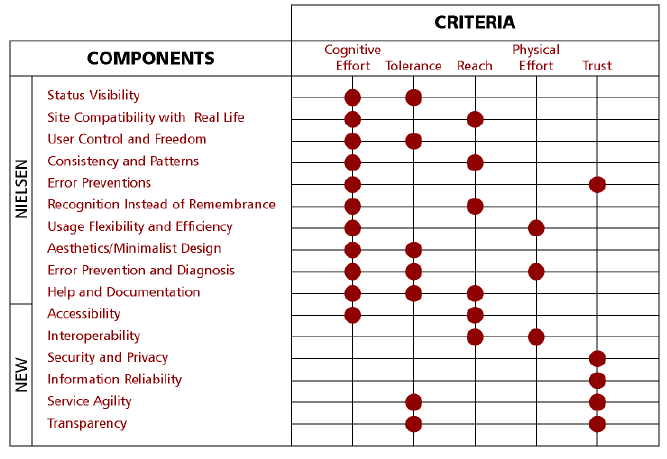
\includegraphics[width=\textwidth]
		{pics/mappinggq.PNG}
	\end{tabular}
	\begin{center}
		{\small Sumber tabel: \citep{paper.garcia}}
	\end{center}
\end{table}
%-----------------------------------------------------------------------------%
\section{\f{Prototyping}}
Dalam mengembangkan produk seorang pengembang pasti memerlukan gambaran ide apa yang ingin dibuat sehingga memerlukan representasi dari ide produk ke bentuk tampilan yang dapat diuji coba dan diubah seiring pengembangan. Metode gambaran proses ide produk ini biasa disebut dengan \f{prototype} . \f{Prototype} merupakan salah satu manifesto desain produk yang memungkinkan pengembang untuk berinteraksi langsung dan mengeksplorasi kesesuainanya secara langsung \citep{buku.preece}. Prototype memiliki banyak bentuk untuk merepresentasikan suatu produk, terdapat juga prototype berdasarkan outline kertas yang merepresentasikan tampilan atau serangkaian tampilan, sebuah gambar elektronik, simulasi video atau rangkaian maket sebagai tampilan mockup keseluruhan rancangan. Prototype digunakan sebagai bantuan dalam mendiskusikan ide antar \f{stakeholders}. Schon (1983) mendeskripsikan bahwa \f{prototype} diakui oleh desainer berbagai ilmu disiplin sebagai sebuah aspek penting dalam proses desain. Prototype menurut \citet{} terbagi menjadi dua jenis, yaitu \f{Low-Fidelity Prototyping} dan \f{High-Fidelity Prototyping}.
%-----------------------------------------------------------------------------%

\subsection{\f{Low-Fidelity Prototyping}}
\f{Low-Fidelity Prototyping} merupakan proses pengembangan desain \f{prototype} yang hasilnya tidak sama dengan produk akhir. Biasanya prototyping ini menggunakan material paper based prototyping atau kardus daripada menggunakan material tampilan elektronik dan metal. Metode ini sangat mudah digunakan karena simpel, cepat dan murah dalam produksinya sehingga sangat sensitif akan perubahan untuk pengubahan desain atau ide. \f{Prototipe} jenis ini dibuat bukan untuk disimpan dan diintegrasikan dengan produk final, dibuat hanya untuk penelusuran ide lebih lanjut. 
\newline\\
\f{Low-fidelity prototyping} terdiri dari jua macam, yaitu storyboard dan sketch. Storyboard merupakan metode prototyping yang menggunakan skenario dalam menjalankannya. Storyboard biasanya tersusun dari sketsa berseri yang menunjukkan bagaimana proses seorang pengguna dalam menjalankan task pada aplikasi. Gambar \ref{fig:story} menjelaskan mengenai seseorang yang menggunakan sebuah sistem baru untuk mendigitalisasi gambar (Hartfield dan Winogard, 1996).

\begin{figure}
	\centering
	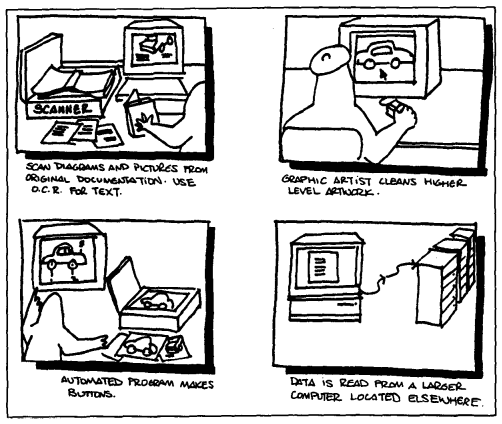
\includegraphics[width=\textwidth]
	{pics/storyboard.PNG}
	\caption{\f{Storyboard} sederhana}
	\label{fig:story}
\end{figure}
\begin{center}
	{\small Sumber gambar: \citep{buku,preece}}
\end{center}
Sketch merupakan metode prototyping yang menggunakan sebuah sketsa dalam menjalankannya, penggunaan metode sketsa dianggap sulit karena banyak yang merasa kurang ahli dalam menggalmbar. Gambar \ref{fig:sketsa} menunjukan sebuah contoh dari sketsa sederhana.
\begin{figure}
	\centering
	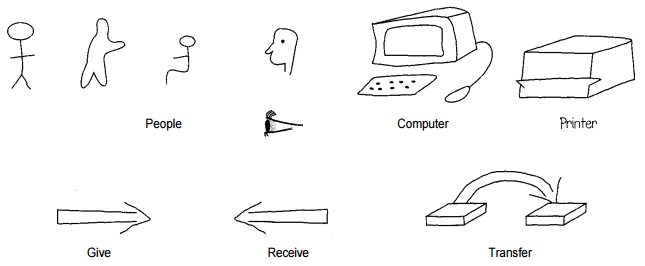
\includegraphics[width=\textwidth]
	{pics/simplesketch.PNG}
	\caption{\f{Sketch} sederhana}
	\label{fig:sketsa}
\end{figure}
\begin{center}
	{\small Sumber gambar: \citep{buku,preece}}
\end{center}
%-----------------------------------------------------------------------------%
\subsection{\f{High-Fidelity Prototyping}}
Perkembangan lebih lanjut dari low-fidelity prototyping adalah high-fifelity prototyping. High-fidelity prototyping biasa digunakan dalam pengembangan produk yang dianggap sebagai produk akhir. Proses pembuatan prototype dibuat dengan material yang diharapkan digunakan dalam produk akhir sehingga produk prototype mirip dengan aslinya. Sebagai contoh produk perangkat lunak yang dikembangkan dengan menggunakan Visual Basic memiliki kesesuaian lebih tinggi dibanding paper-based mockup. High-fidelity prototyping biasanya digunakan untuk menjual ide kepada orang lain dan percobaan terkait kendala teknis. \citet{buku.dyahningrum} menerangkan bahwa metode high-fidelity prototyping digunakan untuk memvalidasi suatu navigasi dengan mental model, mengevaluasi berbagai masalah desain secara mendetail, menggambarkan alur interaksi dan halaman, mengidentifikasi permasalah konsistensi dan berbagai bagian yang berpotensi menjadi masalah teknis.
%-----------------------------------------------------------------------------%
\section{\f{Website} Direktorat Jenderal Pajak}
%-----------------------------------------------------------------------------%
\subsection{\f{Website} Direktorat Jenderal Pajak Indonesia}
%-----------------------------------------------------------------------------%
\subsection{\f{Website} Direktorat Jenderal Pajak India}
%-----------------------------------------------------------------------------%
\section{\f{t-Test}}
%-----------------------------------------------------------------------------%
\section{Aplikasi \f{Web} Proto.io}
%-----------------------------------------------------------------------------%